\section{Fiber Bundle Generation}
\label{subsec:fiber-bundles}
The \mt generated in the previous section represents fragments of fiber bundles. The \mt are clustered in order to extract the final fiber bundles. The clustering process benefits from both the orientation and geometric proximity information inherent in the carbon fiber bundles. Experimentally we found that ``orientation" information was more reliable, while partially overlapping fibers (Figure~\ref{fig:length_distribution}) created problems for ``geometric" proximity based approaches. We also observed that different clustering techniques performed preferably for different measures. 
Instead of creating a heuristic and artificially combining the orientation and geometric proximity measures, we separated the clustering process. 
Specifically, we first cluster based on ``orientation". Each orientation cluster is then further subdivided based on ``geometric" proximity.
The two-step clustering process, helps making the problem more tractable, and the parameters more intuitive to the end users. 
\subsection{Orientation based clustering}
\label {subsec:orientation_clustering}
Before extracting individual fiber bundles, we first separate the \mt into classes based on their major local orientations. To cluster \mt going along similar local directions, we use a spectral embedding technique called Laplacian eigenmaps (originally introduced by Belkin and Niyogi \cite{Belkin01}). An eigenvalue problem is solved to map the manifold embedded in a graph into a lower dimensional space, while preserving the graph structure. 
Let $G$ be the graph, we compute the eigenvalues and eigenvectors for the generalized eigenvector problem $L\textit{\textbf{f}}=\lambda D\textit{\textbf{f}}$,
where $D$ is the diagonal weight matrix and $L$ is the Laplacian matrix. The eigenvector \textbf{${f}_{0}$} corresponding to the eigenvalue 0 is left out and the next $m$, {\textbf{${f}_{1}$} through \textbf{${f}_{m}$}} eigenvectors are used to embed in an $m$-dimensional space (see Sec.~\ref{sec:param_choices} for values of m). 

For our problem, each MetaTract is a node in the graph. We adopt a simple \textit{orientation} based measure to define the weight of the edges. Given a pair of MetaTract, the edge weight between two nodes is defined as the cosine of the maximum angle between the local orientations ($N_P$) of all pairs of start points ($C_P$) between the two MetaTracts. The edge weights give a ``distance matrix" representing the distance between each pair of nodes. Using the Belkin and Niyogi algorithm we ``embed" these nodes in a low dimensional space where the Euclidean distance between nodes, approximates the distance between nodes given by the original ``distance matrix". 
Following this, K-means clustering is employed in the lower dimensional space. Where $K$ is the number of major fiber bundle directions in the woven structure. $K$ is derived from domain knowledge,
for all our test cases, there are two major fiber bundle directions. 
Dimensionality reduction provides us some interesting advantages, by handling the case of curved bundles.
\begin{figure}[t] 
	\centering  	
	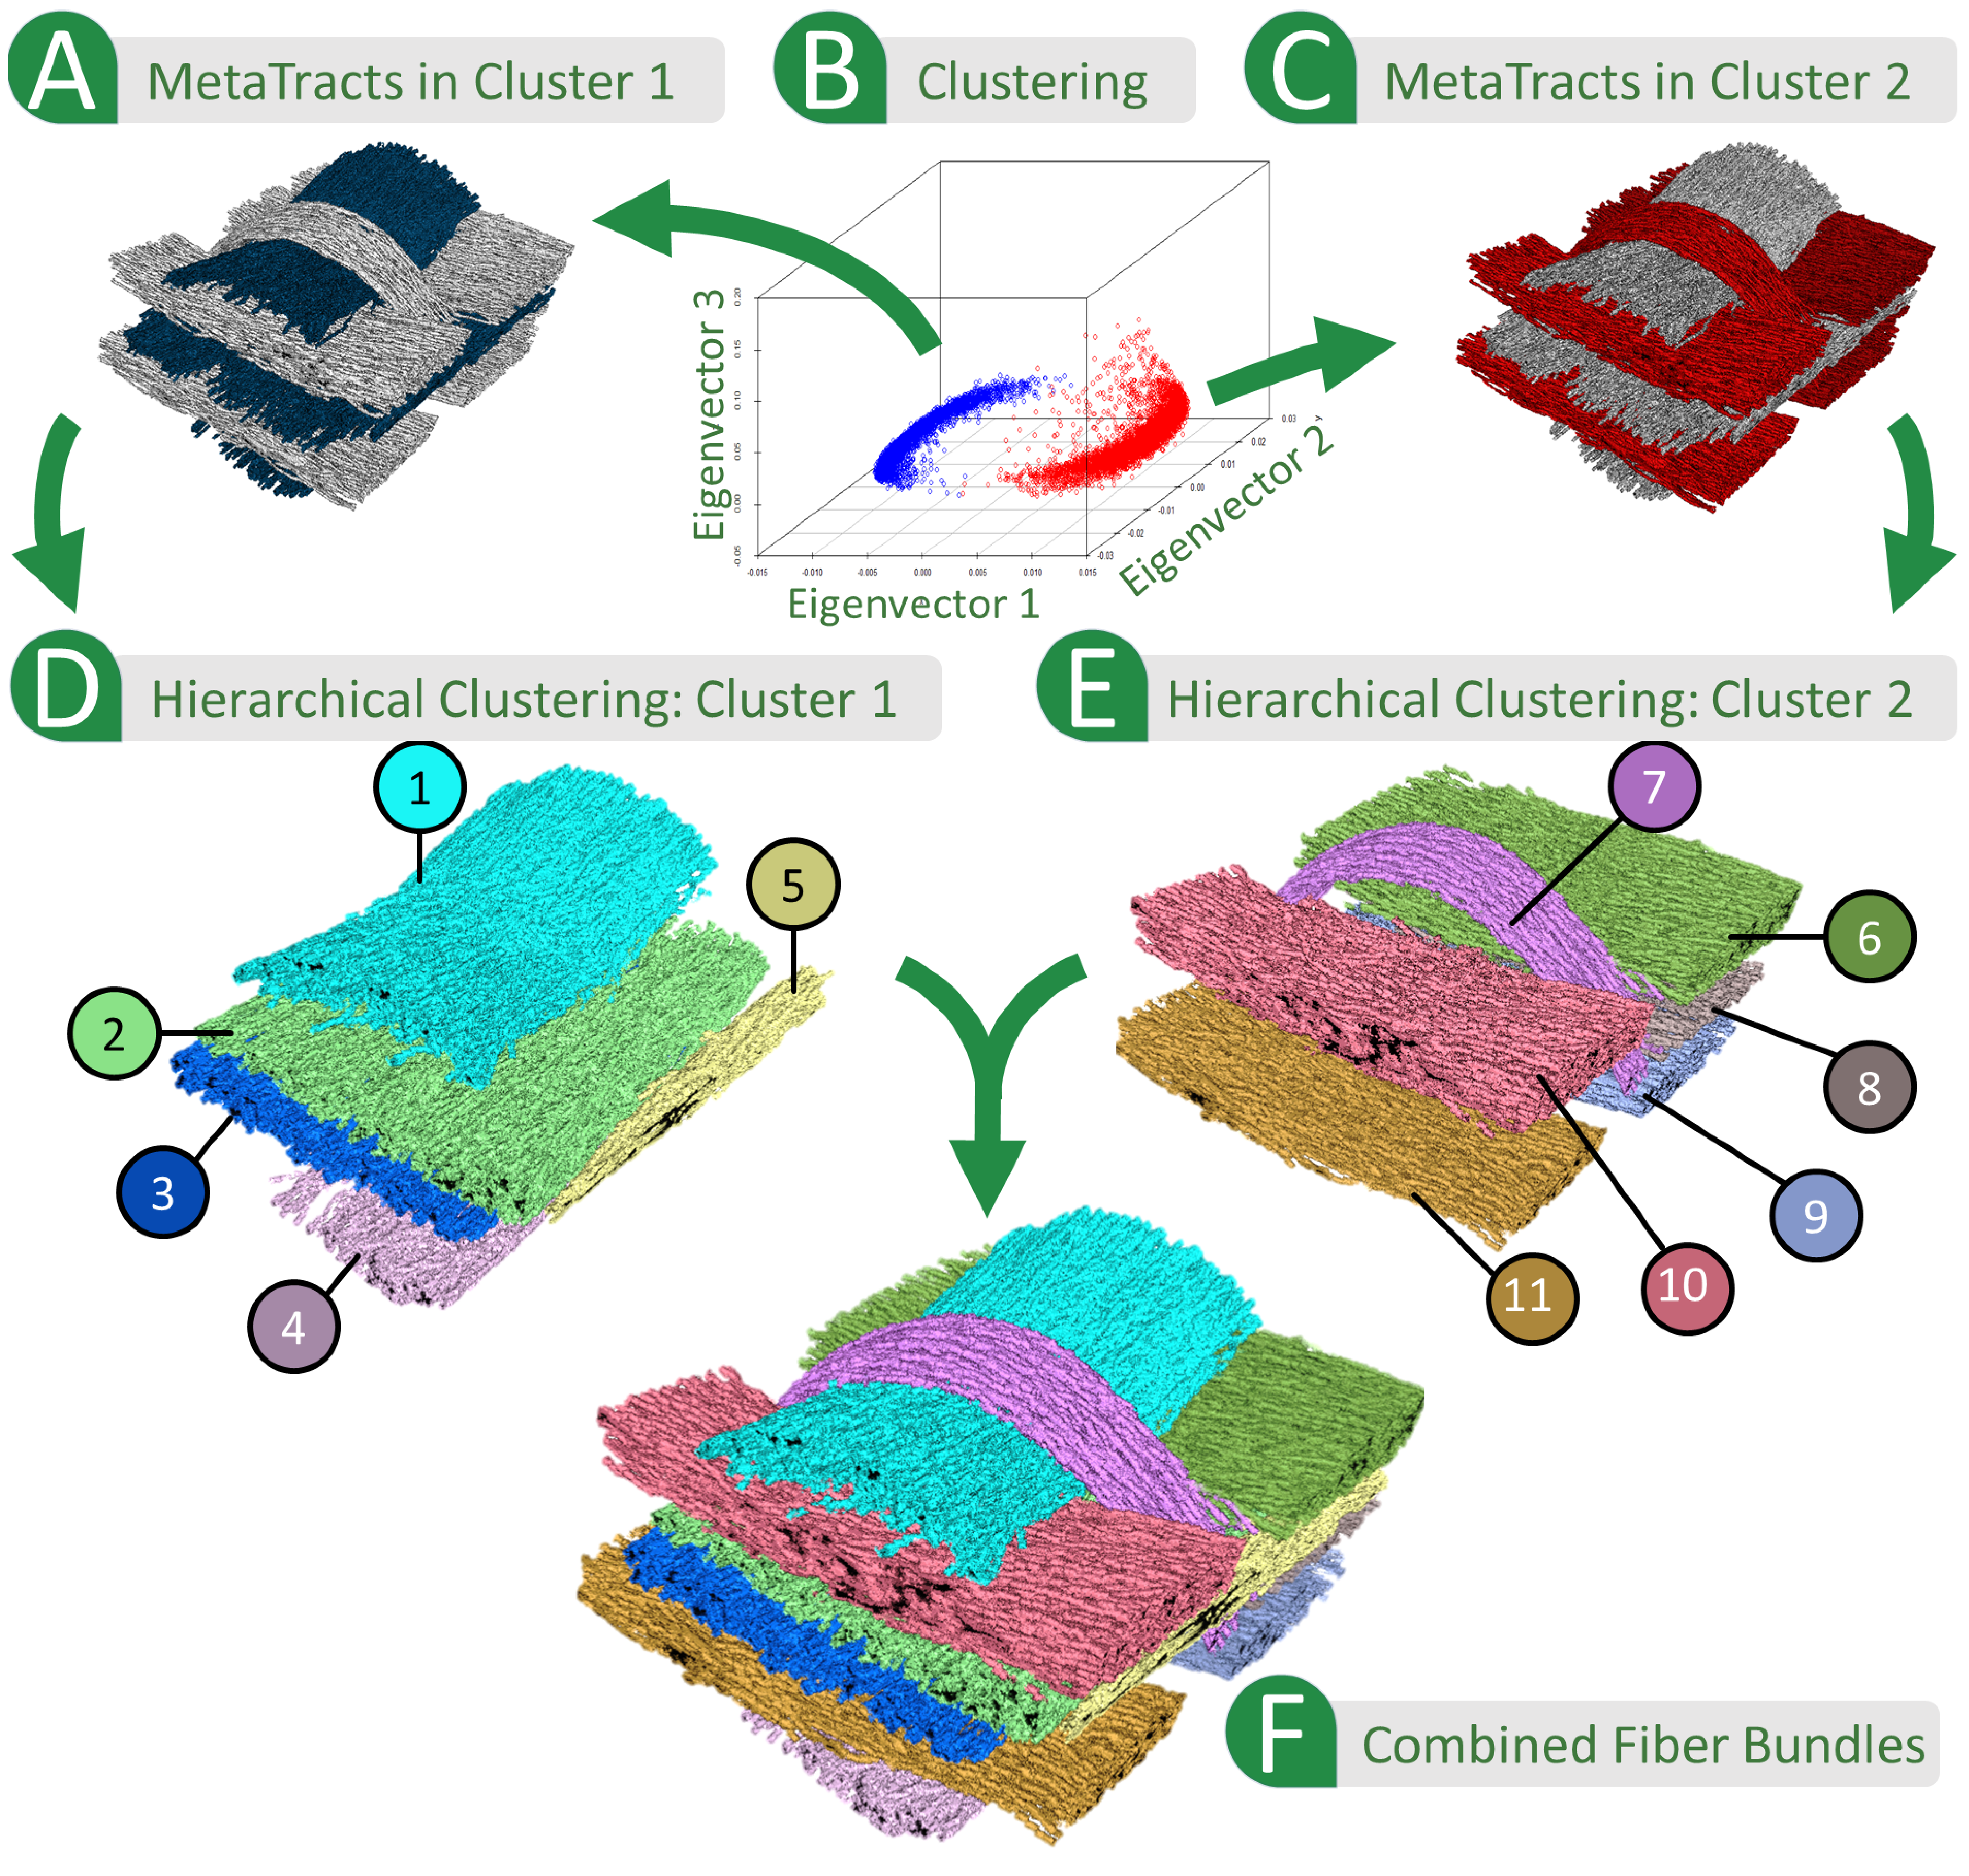
\includegraphics[width=\linewidth]{images/clustering.eps}
	%\includegraphics[width=0.45\textwidth]{imagesMT2014/image_clustering}
	\caption{Clustering Results: Orientation clustering (a,b,c), Distance clustering (d,e).
		 (b) Results of K-means clustering ($K=2$) with \mt (nodes) projected to the top three eigenvectors as major axes. (a) \mt belonging to orientation cluster 1 in blue. (c) \mt belonging to orientation cluster 2 in red, \mt in gray (a,c) show context.
		(d,e) Hierarchical (Distance based) clustering on each orientation cluster. (f) Combined result showing 11 individual extracted clusters. }
	\label{fig:orientation_clustering}
	\vskip-0.2cm
\end{figure} 
Figure~\ref{fig:orientation_clustering}\brac{b} shows the result of the K-means clustering with the nodes (MetaTracts) projected to the top three eigenvectors as the major axes. As expected there is a clear distinction based on fiber bundle orientation. Figure~\ref{fig:orientation_clustering}\brac{a},\brac{c} shows the \mt colored according to orientation clustering results, in blue and red respectively.
Each distinct cluster represents \mt belonging to all fiber bundles, along an individual orientation. 
\subsection{Distance Based Clustering}
\label{subsec:dist_clustering}
To subdivide the oriented clusters into individual fiber bundles, we include further information about the geometric proximity between MetaTracts. We use the directed Hausdorff distance for distance based clustering.
Each MetaTract is represented as a set of points ($C_P$). Formally, the directed Hausdorff distance from point set $P$ to point set $Q$ is defined as 
$H_{dir}(P,Q) = max_{p \in P} min_{q \in Q} d(p,q)$ .
The Hausdorff distance is defined as $H(P,Q) = max(H_{dir}(P,Q),H_{dir}(Q,P))$.
The Hausdorff distance is a metric so $H(P,Q) \le H(P,Q') + H(Q',Q)$ but the directed Hausdorff is not.
%
Unfortunately, the Hausdorff distance does not work well for our application. A single fiber bundle is represented as a set of ``overlapping" MetaTracts. For example  Figure~\ref{fig:length_distribution} shows the length distribution of \mt which express the fiber bundle. Consequently, if a MetaTract $P$ covers only part of the fiber bundle covered by $Q$, then $H_{dir}(P,Q)$ will be very small while $H_{dir}(Q,P)$ will be large.
%
Thus, $H(P,Q)$ will be large, even though $P$ and $Q$ are in the same fiber bundle.
Instead of using the Hausdorff distance, $\max(H_{dir}(P,Q),H_{dir}(Q,P)$, we use $\min(H_{dir}(P,Q),H_{dir}(Q,P))$. If $P$ covers only part of the fiber bundle covered by $Q$, then $\min(H_{dir}(P,Q),H_{dir}(Q,P))$ is very small.
Note that if $P$ and $Q$ overlap but do not cover the same parts of the fiber bundle, then $H_{dir}(P,Q)$ and $H_{dir}(Q,P)$ and $\min(H_{dir}(P,Q),H_{dir}(Q,P))$ will be large.
% 
The directed Hausdorff distance is very sensitive to outliers in the data.
However, because \mt after orientation clustering are constructed using cylinders with similar orientations, they are not plagued by outliers.
To cluster based on MetaTract proximity, we used single linkage hierarchical clustering.
Hierarchical clustering has a single parameter $h$, the desired number of clusters.
Clusters are merged until there are only $h$ clusters left.
Hierarchical clustering is intuitive since it is easy to trace how clusters are formed and merged.
Single linkage clustering finds pairs of objects $p \in P$ and $q \in Q$ where $P \neq Q$ which are closer than other such pairs, and merges the containing clusters $P$ and $Q$.
We found that single linkage hierarchical clustering had two major drawbacks.
\begin{itemize}[nolistsep]
	\item The clustering might produce some ``small" clusters of just a few MetaTracts.
	These \mt are anomalies caused by overlapping fibers and did not represent true fiber bundles.
	\item Second, if two distinct fiber bundles ``ran" parallel for some of their length and then separated, they would sometimes be clustered into a single erroneous bundle.
	This occurs when a short MetaTract which was parallel to both but did not extend into the separation region forms a link between the two fiber bundles. This causes the fiber bundles to be clustered into a single bundle.
\end{itemize}

To address the problem of small clusters, we applied hierarchical clustering and then identified small clusters with few MetaTracts.
We removed the MetaTracts that were in those clusters from the data set and reapplied hierarchical clustering.
To address the problem of short MetaTracts joining different fiber bundles we applied hierarchical clustering and then removed the
shortest tracts (length less than $\eta$ times the median length, set to 0.6) in each bundle. We then reapplied hierarchical clustering.
We repeated both steps until a steady state of clusters was reached and no new small fibers can be removed. The results of hierarchically clustering each orientation cluster ( Figure~\ref{fig:orientation_clustering}\brac{a},\brac{c}) are shown in Figure~\ref{fig:orientation_clustering}\brac{d},\brac{e} respectively.
 
 
After the clustering step, the \mt are separated into well formed fiber bundles. The final result of the clustering process is shown in Figure~\ref{fig:orientation_clustering}\brac{f}. Eleven individual fiber bundles have been separated. Five fiber bundles were extracted from orientation cluster 1 (Z-axis) and six from orientation cluster 2 (X-axis).  
\subsection{Choice of Clustering Techniques}\label{subsec:clus_choice}
\begin{figure}[t]
	\centering
	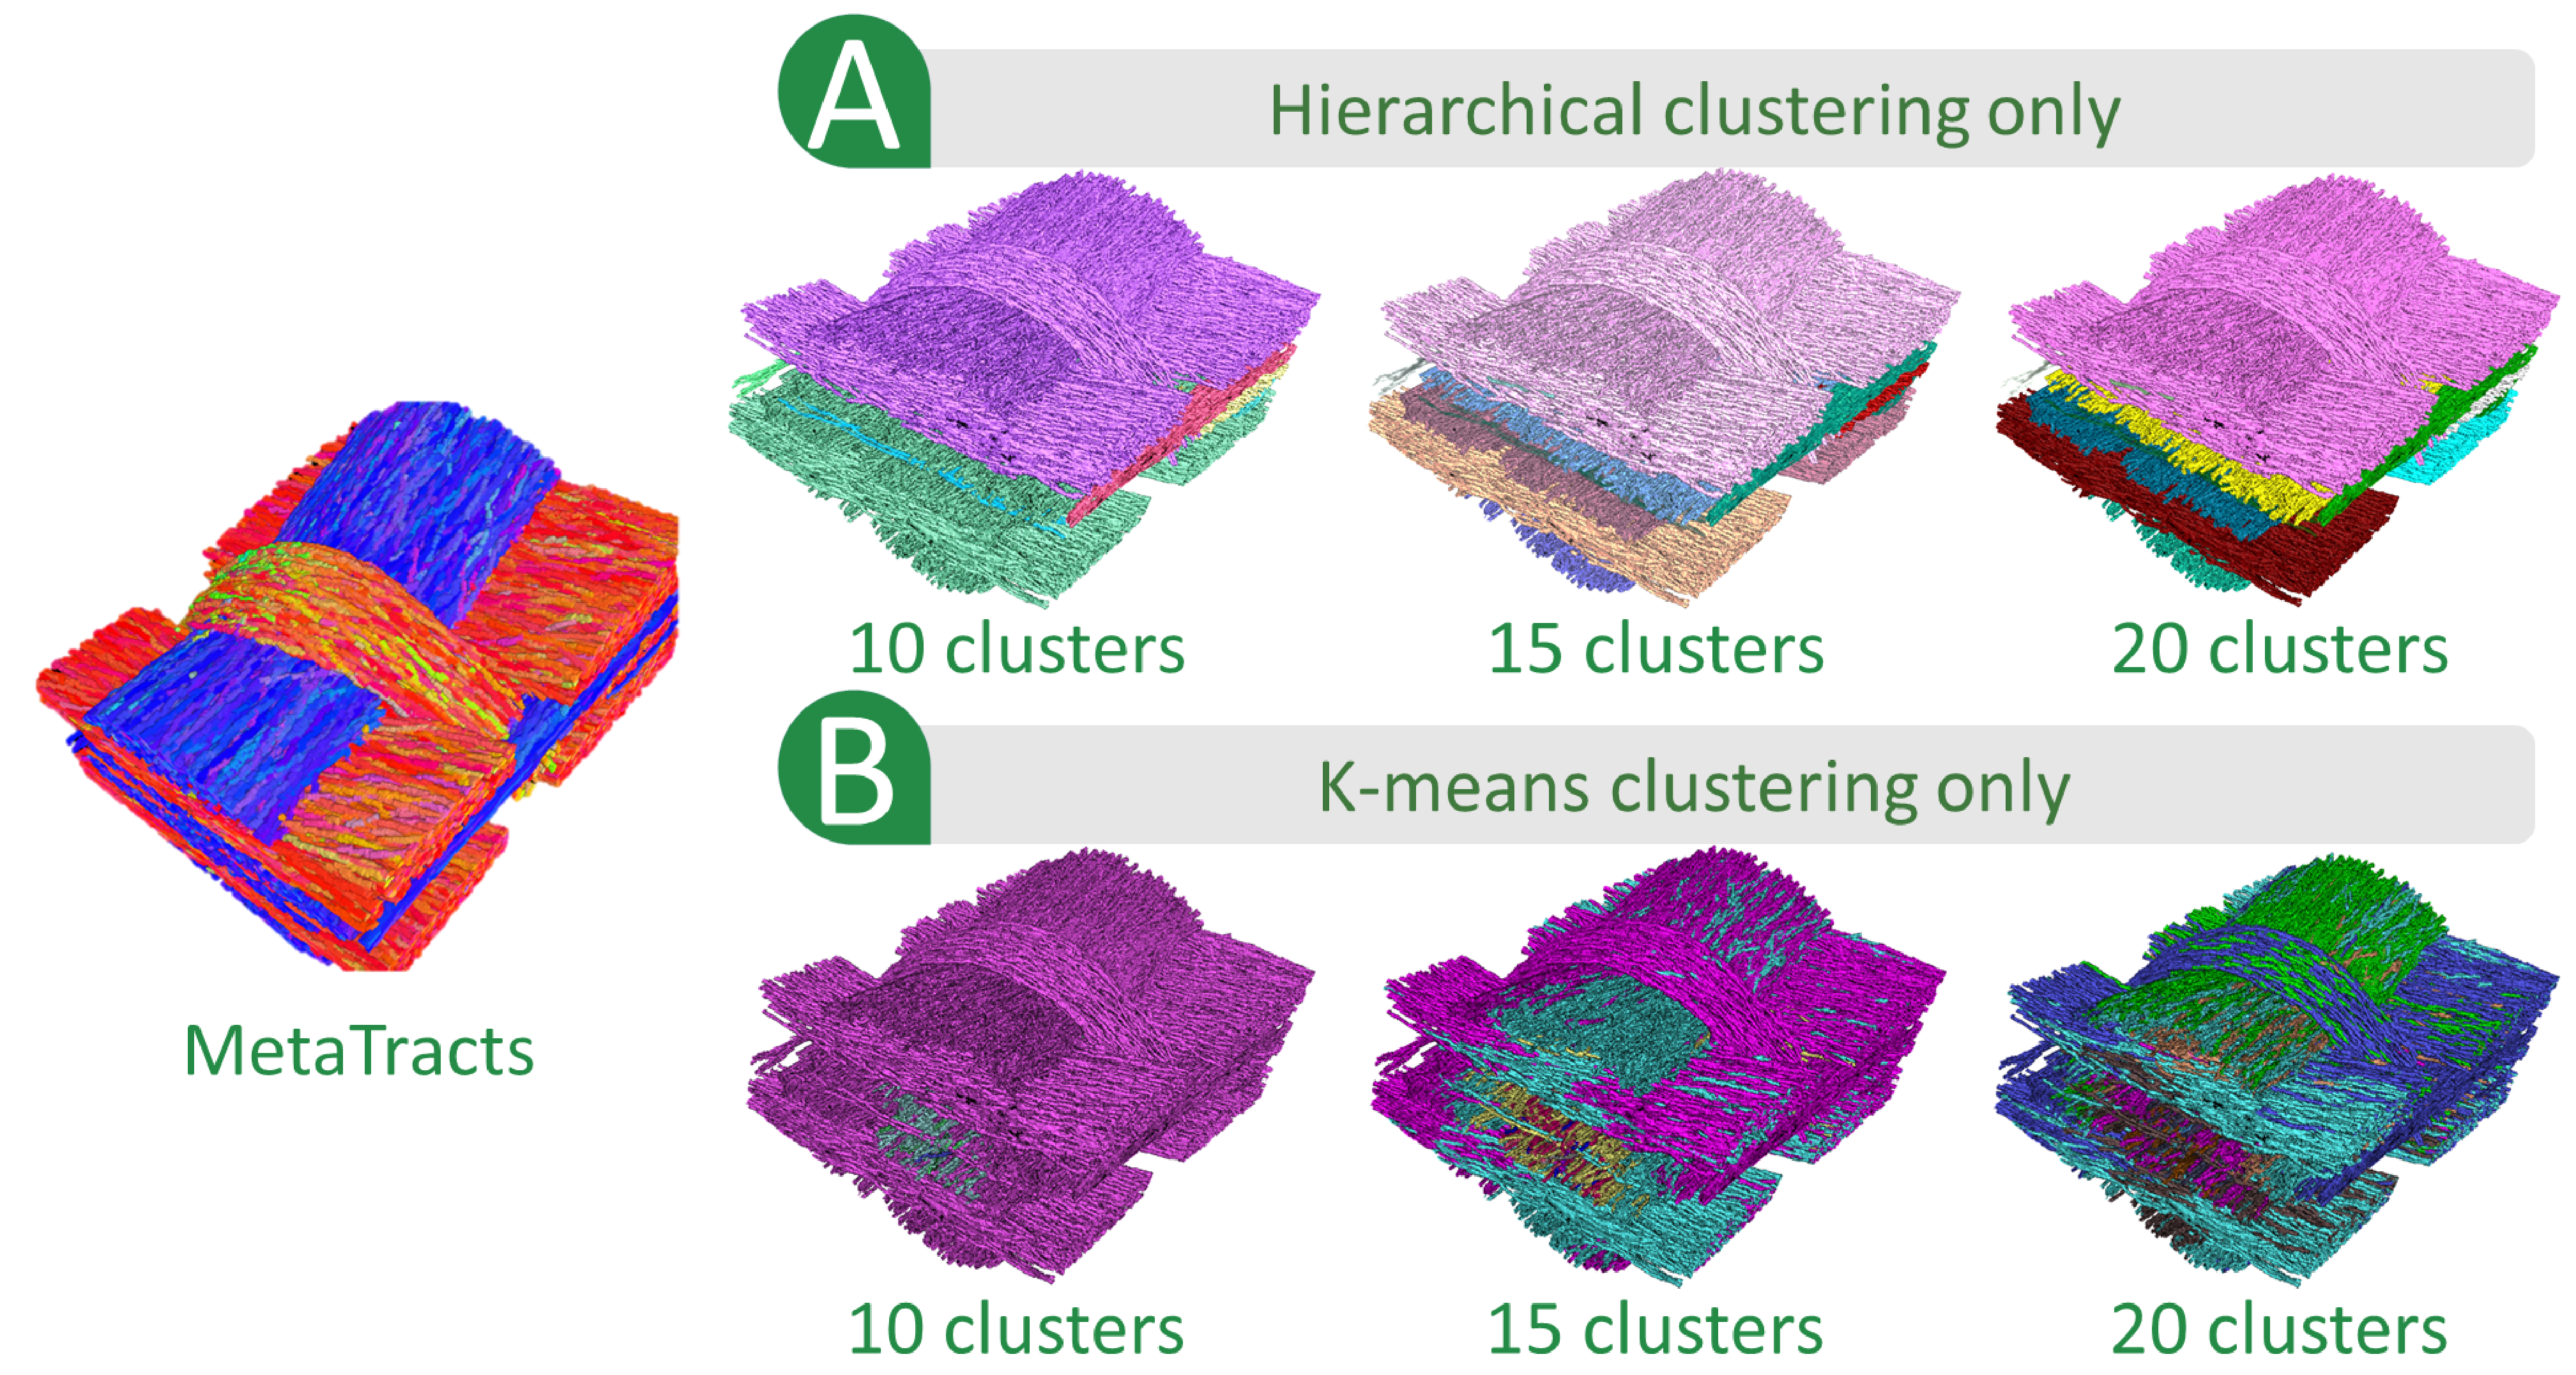
\includegraphics[width=\linewidth]{images/comparison_all.eps}
	\caption{Applying only (a) Hierarchical Clustering and (b) Dimensionality reduction followed by K-means clustering, methods for various numbers of clusters(distance measure is minimal directed Hausdorffs).
		For comparison the results using two-step clustering is in Figure~\ref{fig:orientation_clustering}\brac{f}.}
	\label{fig:comparison}
\end{figure} 
Before settling on the two-step clustering approach, we experimented with using proximity alone, in a single step clustering approach for MetaTracts. We performed two separate tests. First, we used hierarchical clustering to cluster the MetaTracts. Second, we used K-means to cluster the MetaTracts.
Figure~\ref{fig:comparison} shows the results. Figure~\ref{fig:comparison}\brac{a} shows the results of \mt that are hierarchically clustered directly using proximity alone into 10, 15 and finally 20 clusters. 
As discussed in Sec.~\ref{subsec:dist_clustering} single linkage hierarchical clustering in the presence of overlapping \mt tends to create large erroneous clusters and small (low-cardinality) outliers.
When number of clusters (parameter $h$ in hierarchical clustering) is 10, two large incorrect clusters are generated and the rest are outliers. As $h$ increases, some appropriate bundles start to form. But even at $h=20$, fiber bundles incorrectly cluster together. For comparison Figure~\ref{fig:orientation_clustering}\brac{f} shows the two-step clustering result. 


Figure~\ref{fig:comparison}\brac{b} shows the MetaTracts, clustered using K-means clustering by proximity alone, after being embedded in a $m$-dimensional (lower) space. We vary $K$ from 10-20. After the dimensionality reduction, the lower dimensional space does not preserve well the spatial context. As a consequence \mt which are in reality far away are grouped together. Even when k is set to twenty, very few correct fiber bundles are identified.  In comparison, the two-step approach described above is simple, robust and extracts fiber bundles correctly.
\subsection {Sampling \mt}\label{subsec:sampling_mt}
To ensure that the \mt capture the features of all the fiber bundles correctly we uniformly seed the entire volume, which generates a considerably large number of MetaTracts. This increases the time and space requirements of the technique. Especially, orientation clustering which performs eigenvalue and eigenvector computations on large matrices. To ensure that we can handle large datasets and at the same time preserve all features, we start by uniformly seeding the entire volume and generating MetaTracts. We then subsample the \mt and  perform clustering and fiber bundle extraction on these sub-sampled MetaTracts.
The sampling algorithm is given in Algo.~\ref{algo:subsample}. The algorithm  keeps track of a current set of \mt and in each iteration adds the MetaTract furthest from the current set.

Distance between two \mt is measured as the maximum of the minimum distances, between the start points of the cylinders which generate the individual MetaTracts. 
Computing all pairwise distances is an expensive operation. We bound the distances between a MetaTract to others by maintaining a closest set and compute only when necessary.
Note that in step~16 of the algorithm,
we compute the distance from MetraTract $M$
to the newly selected MetaTract $M_i$
only if MetaTract $M_i$ is within distance $2 \times M.dist$ of $M.closest$.
The idea is that if the distance from $M.closest$ to $M_i$ 
is more than $2 \times M.dist$, then $M.closest$ is closer to $M$
than $M_i$ so there is no reason to compute $d(M,M_i)$.

With the sampling step the user can decide the ``resolution" of \mt by setting the parameter $n$ based on their requirements and computational constraints (see Sec.\ref{sec:param_choices}).

\begin{algorithm}[t]
	$S \leftarrow$ set of all \mt\;
	$n \leftarrow$ number of desired \mt\;
	Pick random MetaTract $M_1 \in S$\;
	$S \leftarrow S -\{M_1\}$\;
	\tcc{Initialization: distances and closest bundle.}
	\ForEach{MetaTract $M \in S$}{
		$M.dist \leftarrow$ distance to $M_1$\;
		$M.closest \leftarrow 1$\;
	}
	\For{$i \leftarrow 2$ \KwTo $n$}{
		Pick the MetaTract $M^* \in S$ with largest $M^*.dist$\;
		$M_i \leftarrow M^*$\;
		Compute the distance from $M_i$ to every $M_j$, $j < i$\;
		$S \leftarrow S - \{M_i\}$\;
		\ForEach{MetaTract $M \in S$}{
			$j \leftarrow M.closest$\;
			\If{($d(M_j,M_i) < 2 \times M.dist$)}{
				Compute $dist(M,M_i)$\;
				\If{$(dist(M,M_i) < M.dist)$}{
					$M.dist \leftarrow dist(M, M_i)$\;
					$M.closest \leftarrow i$\;
				}
			}
		}
	}
	\caption{Algorithm to subsample MetaTracts.}
	\label{algo:subsample}
\end{algorithm}

\section{Visualization of \mt}
\label{sec:vis}
The output of the clustering step, can be used to visualize the geometric structure of the fiber bundles and answer the general queries itemized in Sec.~\ref{sec:intro}. Apart from the direct \mt visualization, we added three additional extensions which were requested by the domain specialists as highly important and useful. Specifically, 
\begin{itemize}[noitemsep,nolistsep]
	\item The first extension is to voxelize the original volume according to the clusters each voxel is associated with.
	\item The second extension is to extract surfaces (triangle meshes) associated with each fiber bundle. 
	\item Finally, we added an interactive tool which allows complete visual analysis of the fiber bundles. 
\end{itemize}
\subsection{Voxelization and surface extraction}\label{subsec:voxel_surf_extraction}
To voxelize the entire volume based on the clustering results of the MetaTracts, we take the following ``voting" approach.
We compute a neighborhood around each voxel. We then create a histogram by  enumerating the number of voxels of each class (cluster) in this neighborhood. The voxel is then assigned to the class with the maximum number of elements in the neighborhood. 
Surface extraction is often a crucial requirement for post processing of the data. While Marching Cubes\cite{Lorensen1987} remains the most popular technique, other methods specific to ICT data such as MergeSharp~\cite{Bhattacharya2013} which focuses on extracting sharp edges and corners are also used.  
We extract the corresponding surfaces from voxel data by binarizing the volume per cluster and extracting the isosurface associated with the largest connected component in the input binary volume. 

Figure~\ref{fig:crop-16-decomp}\brac{a} and~\ref{fig:prepreg}\brac{d} show the result of voxelization. Figure~\ref{fig:crop-16-decomp}\brac{b} shows a single slice of the volume along the XY-plane. Figure~\ref{fig:crop-16-decomp}\brac{c},\brac{d} shows examples of extracted meshes.

\begin{figure}[t]
	\centering
	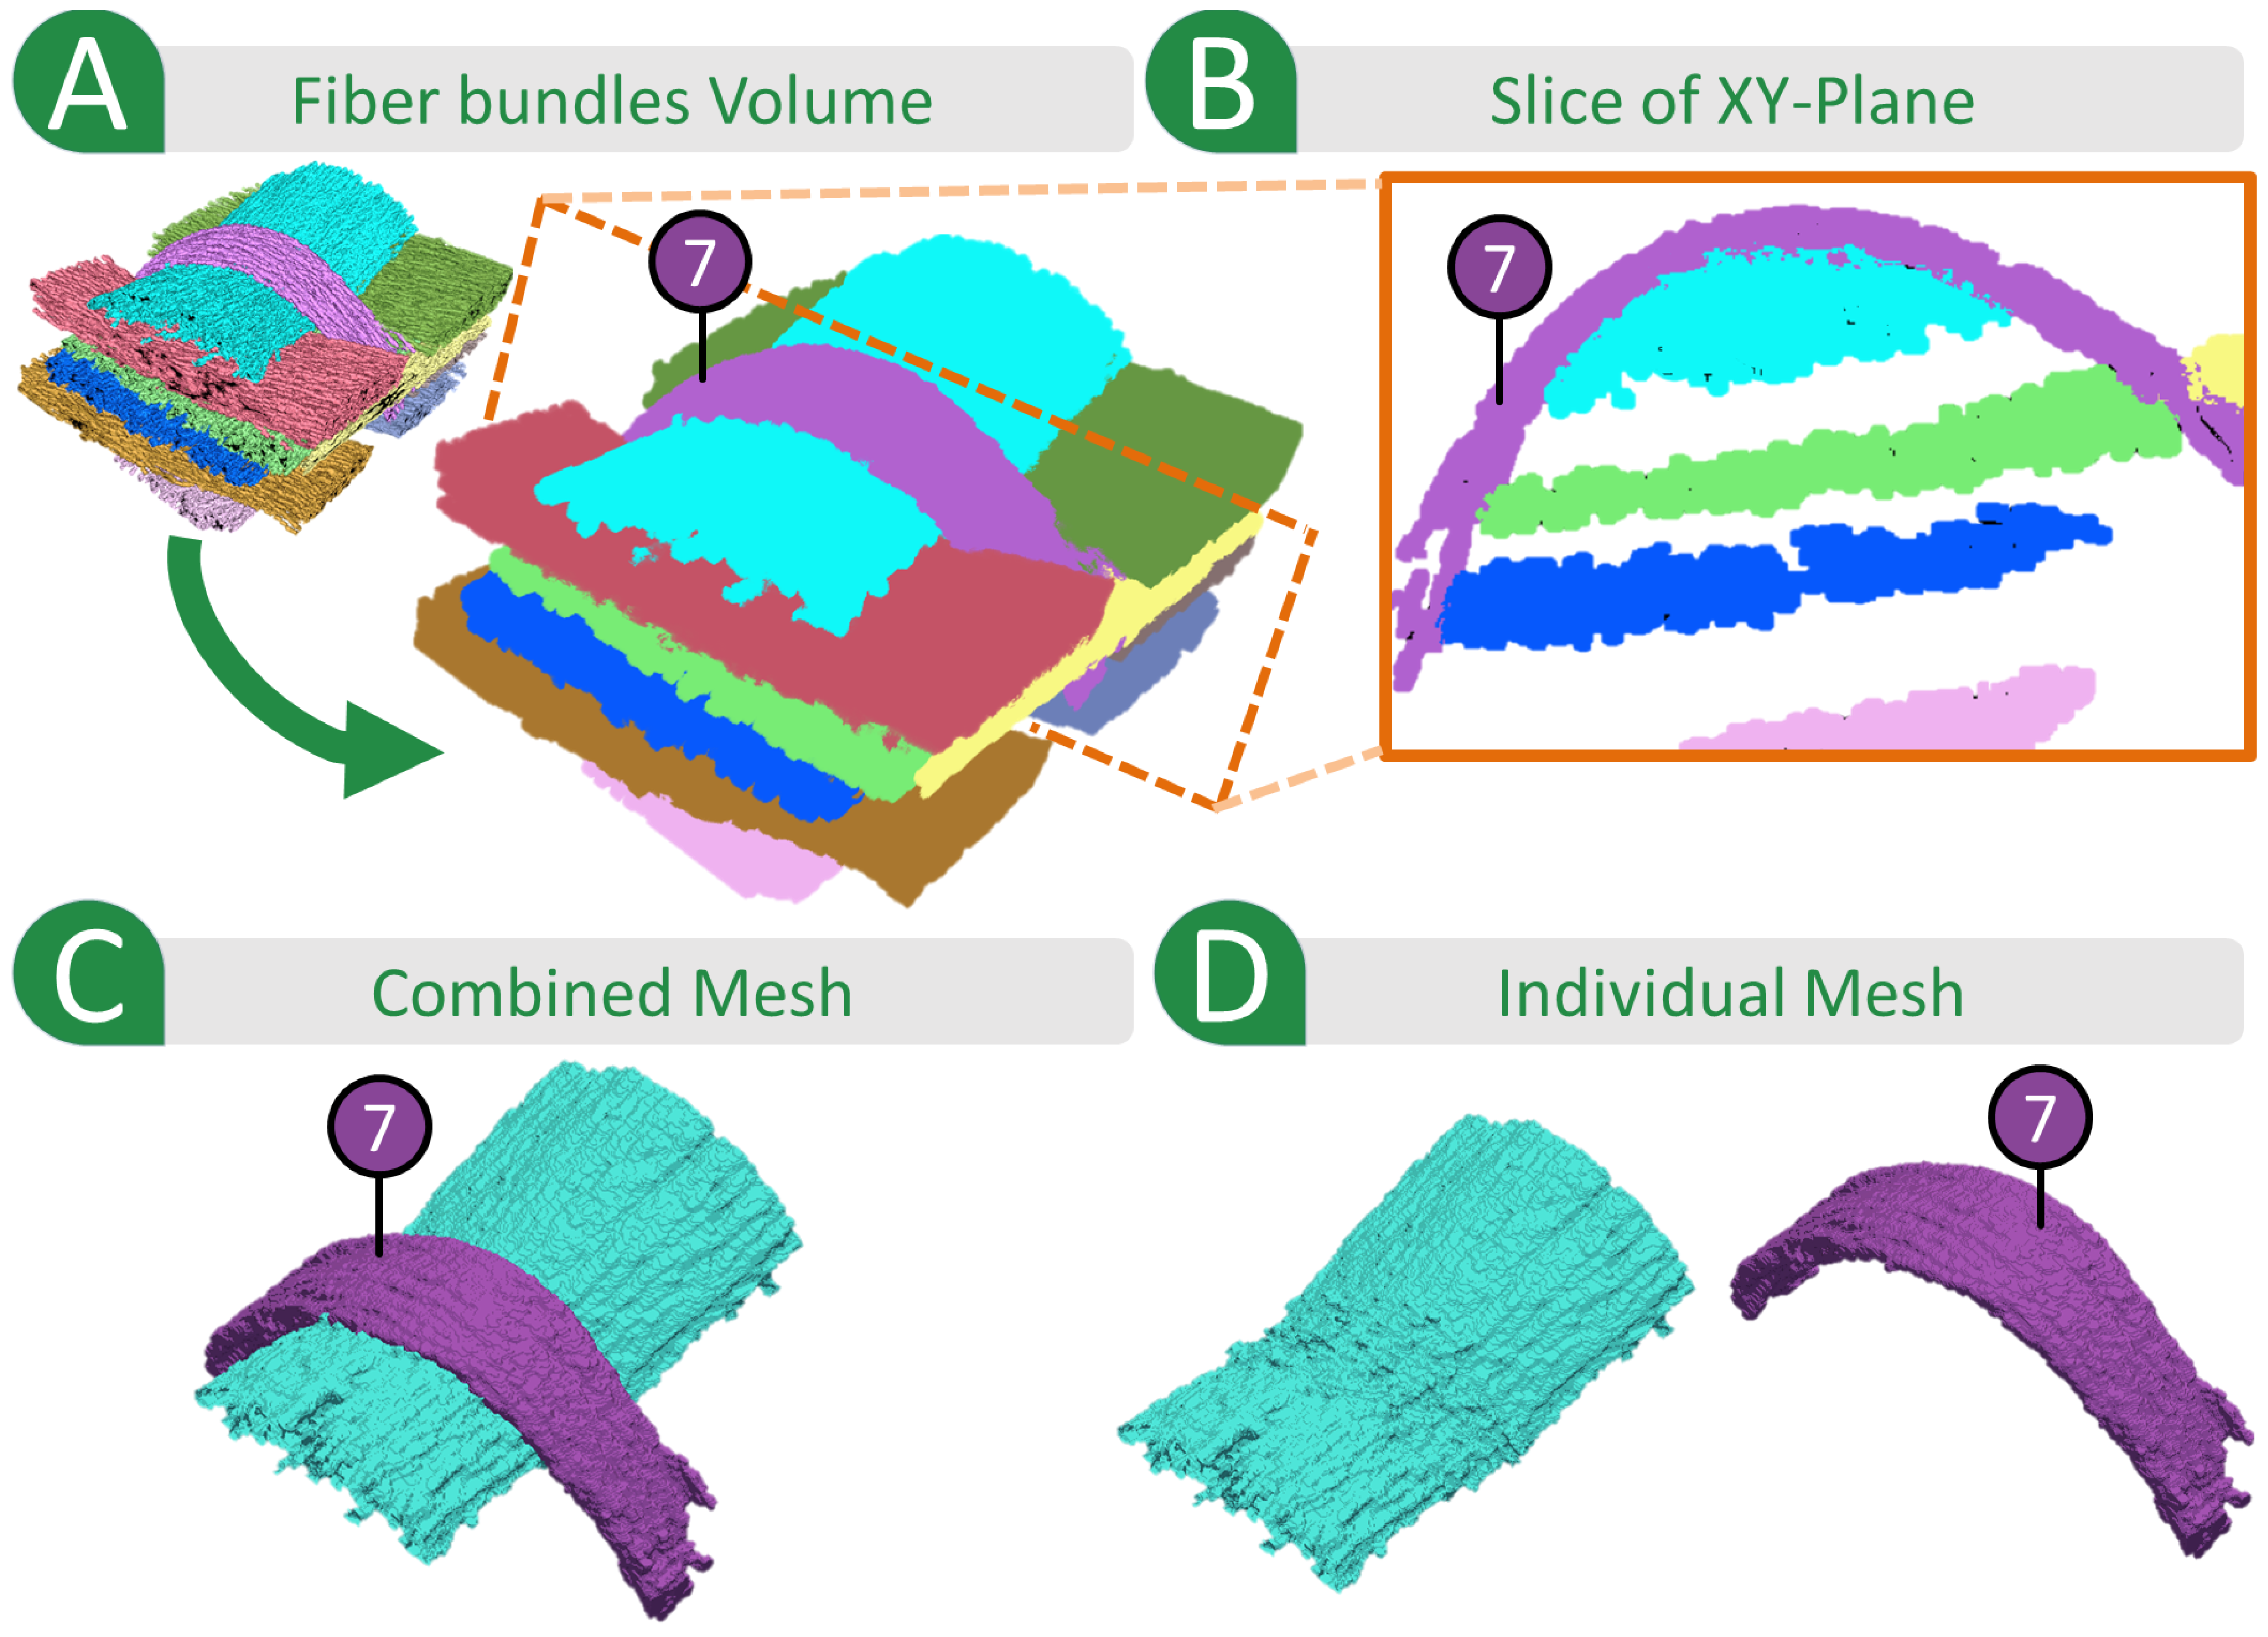
\includegraphics[width=\linewidth]{images/figure8.eps} 
	\caption{Voxelization and surface extraction. (a) Voxelization of data set 1, the inset shows the \mt after clustering. (b) a single slice along the XY-Plane (c) Two of the extracted meshes together (d) The meshes rendered separately.}
	\label{fig:crop-16-decomp}
\end{figure} 



